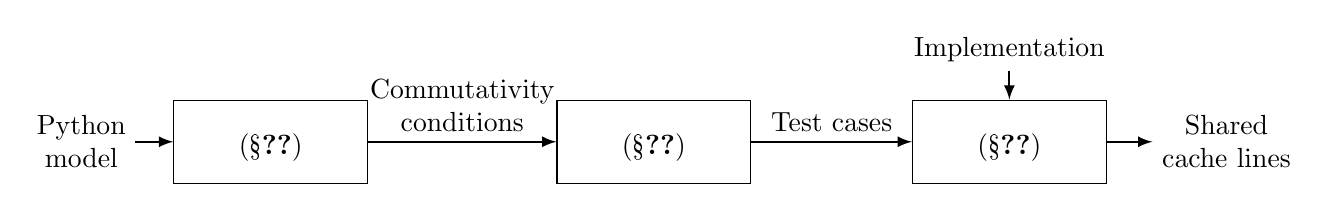
\begin{tikzpicture}[>=latex]

\tikzstyle{pass} = [draw, rectangle, align=center, minimum height=3em, minimum width=7em]
\tikzstyle{inout} = [align=center];
\tikzstyle{edge} = [draw, thick, ->];
\tikzstyle{data} = [align=center, midway, anchor=south];
\tikzstyle{none} = [node distance=6.8em];

\node[inout, name=beg] {Python \\ model};
\node[pass, name=ana, right of=beg, xshift=4em] {\analyzer \\ (\S\ref{sec:tool:analyzer})};
\node[pass, name=gen, right of=ana, xshift=11em] {\testgen \\ (\S\ref{sec:tool:generator})};
\node[pass, name=mtr, right of=gen, xshift=10em] {\mtrace \\ (\S\ref{sec:tool:mtrace})};
\node[inout, name=imp, above of=mtr, yshift=.5em] {Implementation};
\node[inout, name=end, right of=mtr, xshift=5em] {Shared \\ cache lines};

\draw[edge] (beg) -- (ana);
\draw[edge] (ana) -- (gen) node[data] {Commutativity \\ conditions};
\draw[edge] (gen) -- (mtr) node[data] {Test cases};
\draw[edge] (mtr) -- (end);
\draw[edge] (imp) -- (mtr);

\end{tikzpicture}
